%%%%%%%%%%%%%%%%%%%%%%%%%%%%%%%%%%%%%%%%%%%%%%%%%%%%%%%%%%%%%%%%%%%%%%%%%%%%%%%%
%2345678901234567890123456789012345678901234567890123456789012345678901234567890
%        1         2         3         4         5         6         7         8

\documentclass[letterpaper, 10 pt, conference]{ieeeconf}  % Comment this line out if you need a4paper

%\documentclass[a4paper, 10pt, conference]{ieeeconf}      % Use this line for a4 paper

\IEEEoverridecommandlockouts                              % This command is only needed if 
                                                          % you want to use the \thanks command

\overrideIEEEmargins                                      % Needed to meet printer requirements.

% See the \addtolength command later in the file to balance the column lengths
% on the last page of the document

% The following packages can be found on http:\\www.ctan.org
%\usepackage{graphics} % for pdf, bitmapped graphics files
%\usepackage{epsfig} % for postscript graphics files
%\usepackage{mathptmx} % assumes new font selection scheme installed
%\usepackage{times} % assumes new font selection scheme installed
%\usepackage{amsmath} % assumes amsmath package installed
%\usepackage{amssymb}  % assumes amsmath package installed
\title{\LARGE \bf
Modular Task and Motion Planning in Belief Space 
}


\author{Dylan Hadfield-Menell$^{1}$, Edward Groshev$^{2*}$, Rohan Chitnis$^{2*}$, and Pieter Abbeel$^{1}$% <-this % stops a space
\thanks{$^{1}$\{\tt \small dhm, pabbeel\}@eecs.berkeley.edu}%
\thanks{$^{2}$\{\tt \small eddiegroshev, ronuchit\}@berkeley.edu}%
\thanks{\normalsize{\textit{* denotes equal contribution among these authors}}}%
}

%% \usepackage[numbers]{natbib}
\usepackage{multicol}
\usepackage[bookmarks=true]{hyperref}
\usepackage{color}
\usepackage{amssymb}
\usepackage{amsmath}

%% \usepackage{amsthm}
\usepackage{booktabs}
\usepackage{graphicx}

\usepackage{caption}
\usepackage{subcaption}
%%\usepackage{subfigure}

\usepackage{algorithm}
\usepackage{algpseudocode}


\DeclareMathOperator*{\argmin}{argmin}
\DeclareMathOperator*{\argmax}{argmax}

\newenvironment{tightlist}%
{\begin{list}{$\bullet$}{%
    \setlength{\topsep}{0in}
    \setlength{\partopsep}{0in}
    \setlength{\itemsep}{0in}
    \setlength{\parsep}{0in}
    \setlength{\leftmargin}{1.5em}
    \setlength{\rightmargin}{0in}
    \setlength{\itemindent}{-.1in}
}
}%
{\end{list}
}

% \setlength{\parskip}{1pc}
% \setlength{\parindent}{0pt}
% \setlength{\topmargin}{-3pc}
% \setlength{\textheight}{9.5in}
% \setlength{\oddsidemargin}{0pc}
% \setlength{\evensidemargin}{0pc}
% \setlength{\textwidth}{6.5in}

\newcommand{\secref}[1]{Section~\ref{#1}}
\newcommand{\exref}[1]{Example~\ref{#1}}
\newcommand{\eqnref}[1]{Equation~\ref{#1}}
\newcommand{\figref}[1]{Figure~\ref{#1}}
\newcommand{\algoref}[1]{Algorithm~\ref{#1}}

\newcommand{\dhm}[1]{{\bf \textcolor{red}{Dylan: #1}}}

\newtheorem{thm}{Theorem}
\newtheorem{lem}{Lemma}
\newtheorem{defn}{Definition}
\newtheorem{conj}{Conjecture}
\newtheorem{cor}{Corollary}
\newtheorem{ex}{Example}
 
\newcommand{\ibsp}{\textsc{ibsp}}

\newcommand{\aml}{\textsc{aml}}
\newcommand{\mld}{\textsc{mld}}

\newcommand{\E}{\mathcal{E}}
\newcommand{\F}{\mathcal{F}}
\newcommand{\Ops}{\mathcal{A}}


\begin{document}

\bibliographystyle{IEEEtran}

\maketitle
\thispagestyle{empty}
\pagestyle{empty}


%%%%%%%%%%%%%%%%%%%%%%%%%%%%%%%%%%%%%%%%%%%%%%%%%%%%%%%%%%%%%%%%%%%%%%%%%%%%%%%%
\begin{abstract}
The execution of long-horizon tasks under uncertainty is a fundamental
challenge in robotics. Recent approaches have made headway on these
tasks with an integration of task and motion
planning.  In this paper, we present Interfaced
Belief Space Planning (\ibsp), a modular approach to task and motion
planning in belief space. We use a task-independent interface layer to
combine an off-the-shelf classical planner and motion planner, enabling us to
solve complex problems in belief space. We determinize
the problem under the maximum likelihood observation assumption to obtain a
deterministic representation that can generate reasonable information-seeking
behavior. We leverage properties of maximum
likelihood determinizations to utilize a simple representation of
(optimistic) belief space dynamics that is well-suited to
planning. Our interface can be implemented with standard belief state
queries, requiring only the ability to sample, compute unnormalized
likelihoods, and answer maximum likelihood queries. Our contribution
is a novel algorithm for task and motion planning in belief space. The
algorithm is a novel approach that substantially reduces dependence on details of the belief
state dynamics. \ibsp{} can work with a broad class of black box state
estimators, with zero changes to the algorithm. We show that \ibsp{} is
complete for a (restricted) class of partially observable problems. We
validate our approach in simulated tasks for the PR2 that account for
continuous state, different belief distributions, and negative observations.
\end{abstract}



%%%%%%%%%%%%%%%%%%%%%%%%%%%%%%%%%%%%%%%%%%%%%%%%%%%%%%%%%%%%%%%%%%%%%%%%%%%%%%%%
\section{INTRODUCTION}
A central goal in robotics is the execution of long-horizon tasks in
the face of uncertainty. Any reader that has spent frantic mornings
searching for lost keys understands the challenges such problems
present. Completing such a task corresponds to reasoning about
multimodal belief distributions where obtaining an observation
can require long, temporally extended plans. 
\begin{figure}[h]
  \centering
    \noindent
    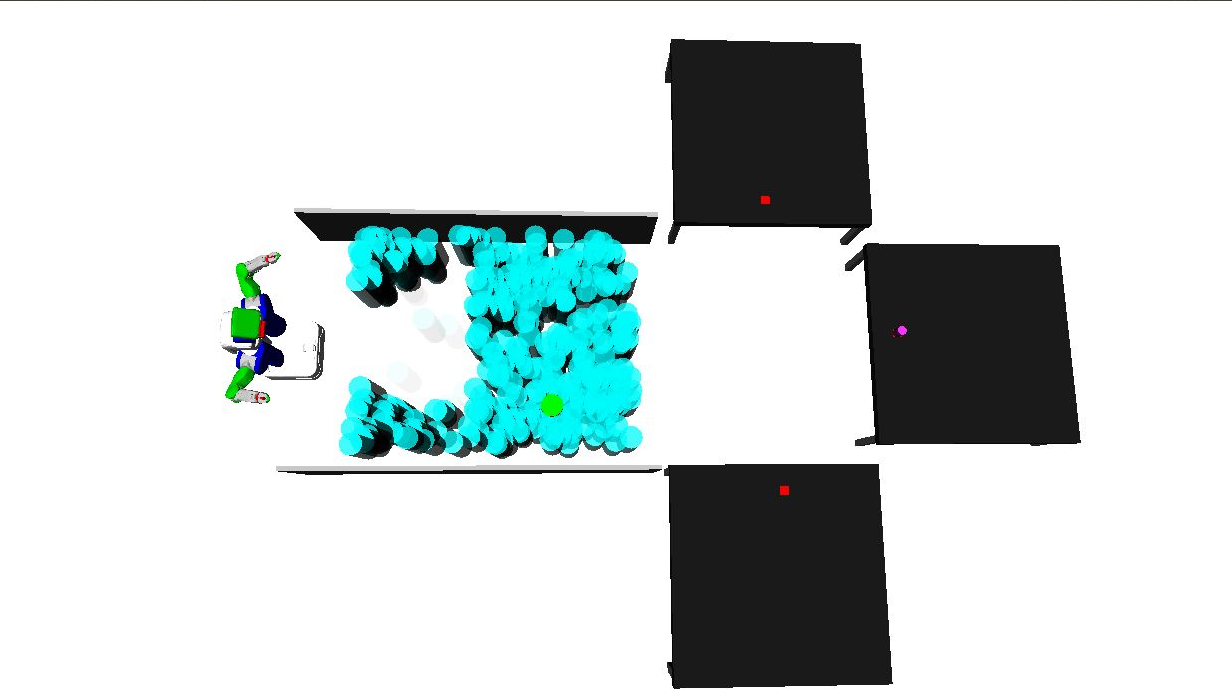
\includegraphics[width=0.45\textwidth]{corridor_images/obj_at_true_loc.png}
  \caption{A screenshot from one of our experiments. The robot is
    tasked with navigating to the other side of the corridor, but
    there is a uniform distribution of obstacles in the way. Our low
    level refinement algorithm detects the probability of obstruction and
    propagates information to the high level. The objects shown are
    from the posterior distribution after a single negative
    observation.}
  \label{fig:knot_steps}
\end{figure}


Discovering a solution to this task necessitates finding a policy that
accounts for uncertainty in locations of objects, locations of the
robot and non-determinism in the dynamics (among other
challenges). Solving such problems exactly is far beyond the state of
the art in partially observable Markov decision processes.

Given the intractability of this problem, how can we hope to make
progress? Our starting point takes inspiration from recent methods for
fully observed task and motion planning.  This is a challenge in its
own right, but careful applications of abstraction, lazy
discretization, and motion planning have made inroads on this
problem~\cite{srivastava2014combined, lozano2014constraint}. These
approaches plan in an \emph{abstract} representation of a problem
(without continuous variables) and use sampling and motion planning to
\emph{refine} abstract plans into fully grounded plans involving continuous
operators.

A key insight is that many of the difficulties in planning with belief
states, which are inherently continuous, are shared by the continuous
state-action spaces for task and motion planning. This suggests a
strategy that applies similar abstraction techniques to belief state
representations of a planning problem.

Another important development is that of \emph{maximum
likelihood determinizations} (\mld) of
POMDPs~\cite{platt2010belief}. This approximation assumes that each
belief state produces its maximum likelihood observation. The result
is a deterministic problem that encourages reasonable information-gathering
behavior. It is amenable to suitably modified standard
methods; these methods typically prescribe solving a complex,
continuous, under-actuated problem. However, integration with task
planners provides relief from this problem---high level tasks can
split a low-level problem into an observe phase and a motion phase
(which is the output of joint solution methods in many scenarios).

We present an algorithm, Interfaced Belief Space Planning (\ibsp),
that leverages these insights. It extends the domain abstraction techniques from
Srivastava et al.~\cite{srivastava2014combined} to \mld{} formulations of large continuous
POMDPs. We leverage properties of an \mld{} to construct a simple high-level
representation of belief states so that (optimistic) belief
state dynamics are compactly represented. The algorithm alternates
among extracting a plan skeleton, assigning values to continuous
variables, and updating the high level with failure information if a
refinement can not be found.
\ibsp{} enforces a clear separation among extracting plan skeletons
from a domain description, refining a plan skeleton, and determining
success or failure of a plan; furthermore, each component relies on
standard operations. Our implementation uses off-the-shelf classical
planners to generate plan skeletons and sampling and trajectory
optimization to generate refinements. 

Our refinement strategy only requires the ability to compute maximum
likelihood observations for a belief state and the ability to filter
beliefs. We detect plan failure and propose state updates with Monte Carlo
sampling. Such structured access to the belief state allows \ibsp{} to work with a broad class
of beliefs with minimal algorithmic changes. While our high-level
planner uses an abstract belief representation, the full algorithm
plans with the true belief dynamics and is capable of generating and executing plans
with complex state estimation methods. We validate our approach in
partially observable mobile manipulation tasks with a variety of
belief distributions that account for negative observations, such as object retrieval from
one of many possible drawers and navigation through a corridor containing several objects
whose locations are only initially known to be in a uniform distribution over the corridor. We
present formal results showing completeness for a subclass of POMDPs.

%%PA: it'd be really good to include specifics about the
%%scenarios in which we evaluate our approach and specifics about the 
%% behaviors it manages to generate;   for many readers
%%interesting scenarios will make them interested in the approach,
%%lack thereof will make them wonder why they would bother reading
%%this paper...


%%PA: can we have a representative teaser figure on the first page
%%(top of the right column) ?

\section{Related Work}
Our work builds on recent results in deterministic task and motion
planning. Early work in task and motion planning was embodied in the
aSyMov system~\cite{gravot2005asymov}, where a task plan was generated
and used to guide motion planning. However, the focus was on
determining a way to solve motion plans in parallel. Dornhege et
al. use semantic attachments to do task and motion planning with
classical planners~\cite{dornhege2012semantic}. This approach makes
use of task planners, but requires representation of discretized
locations within the high level. Havur et al. use local search to find
an optimal geometric configuration before discretizing the continuous
plane into non-uniform cells and using a hybrid planner to find a
feasible motion plan~\cite{havur2014geometric}. Lagriffoul et
al. parameterize symbolic actions with coarse geometric
representations of objects and grasp types. Possible geometric
instances are sampled from the symbolic plan and are pruned by
constraints to reduce geometric
backtracking~\cite{lagriffoul2014orientation}.

Maximum likelihood determinization was introduced by Platt et
al.~\cite{platt2010belief}. They used this approach to frame problem
solving in belief space as an underactuated control problem. They use
LQR and transcription methods to find trajectories in belief space and
characterize scenarios where a replanning strategy is guaranteed to
succeed. Van Den Berg et al. use LQG to solve Gaussian belief space
planning problems that incorporate collision avoidance
constraints~\cite{van2012motion}. They are able to plan without
the maximum likelihood assumption and explore the approximations
introduced with maximum likelihood determinizations.
 
Our determinization-replan approach shares similarity with
determinization-replan approaches for probabilistic planning, such as
FF-replan~\cite{yoon2007ff}. Both leverage determinization in order to
obtain major performance gains from classical planners. The maximum
likelihood assumption is similar to the most likely transition
determinization from that literature, while our optimistic belief
updates are similar to an all outcomes determinization.
 
The idea of using knowledge space representations is an old idea in
artificial intelligence that dates back to McCarthy and
Hayes~\cite{mccarthy1968some}. Bonet and Geffner provide in-depth
experimentation and analysis of discrete deterministic partially
observed planning~\cite{bonet2011planning}.  They provide conditions
under which discrete formulations of partially observable planning
(with binary, factored beliefs) can be compiled to sound and complete
representations. The conditions for this are similar to conditions for
our completeness theorem; however, our algorithms are aimed at large
continuous problems for robotics while their work is aimed at
classical planning.

% Our approach relies on the maximum likelihood determinization
% introduced by Platt et al.~\cite{platt2010belief}. They frame problem
% solving in belief space as an underactuated control problem and apply
% continuous techniques. 

The Belief Space Hierarchical Planning in the Now (BHPN) planning and execution system is a task and motion planning
approach to handle uncertainty~\cite{kaelbling2013integrated}. Similar
to our approach, they construct task plans in belief space under
maximum likelihood determinization. Levihn et al. extend this system
to construct shorter plans at execution time by smart replanning and
reconsideration~\cite{levihn2013foresight}. They explicitly formulate
the regression of belief goals under Gaussian distributions and plan
with an exact representation of belief state dynamics. In contrast, we
use references to the belief so we can plan with arbitrary belief
representations, not just Gaussians.

Srivastava et al. formulate open world \pomdp s with a probabilistic
program~\cite{srivastava2014first} -- they develop a generalization of
point-based value iteration to that setting. While both our method and
theirs can been viewed as solving very large \pomdp s, their method's size stems from
the (unbounded) size of the world and complexity of corresponding
beliefs, while ours stems from uncertainty about continuous quantities.


Gashler et al. use a contingent planner to generate plans that react
to feedback from the world~\cite{gaschler2013kvp}. They generate
contingent plans and use external function calls during their planning
step to generate effects of actions. However, they explicitly
represent poses and belief updates in symbolic models for task
planning. We use pose and belief references to plan abstractly. We
refine and verify plans with the \emph{true} belief.

Nebel et al. use a three valued logic for the TidyUp project that
allows fluents to take the value
\emph{uncertain}~\cite{nebel13aaaiirs}. In their system, however, they
assume that uncertain items become known once the robot is close
enough and so do not explicitly plan sensing actions. In contrast, we
represent uncertainty directly and combine
reasoning about uncertainty with reasoning about maximum likelihood
states.

%% Our determinization-replan approach shares similarity with
%% determinization-replan approaches for probabilistic planning, such as
%% FF-replan~\cite{yoon2007ff}. Both leverage determinization in order to
%% obtain major performance gains from classical planners. The maximum
%% likelihood assumption is similar to the most likely transition
%% determinization from that literature, while our optimistic belief
%% updates are similar to an all outcomes determinization.


\section{Technical Background}
\subsection{Observable planning formulation}
\label{sec-formulation}
We use a STRIPS-style formalism to define our planning problems. We
introduce a simple pick and place task that will serve as a running
example for the paper. 

Formally, we define a (fully observed) planning problem, $\Pi$ as a tuple, $\Pi =
\langle \E, \F, I, G, \Ops \rangle$, with the following definitions:
\begin{tightlist}
\item[$\E$:] a set of \emph{entities} within our domain; e.g. individual objects or locations.
\item[$\F$:] a set of \emph{fluents} that describe relations between
  entities.
\item[$I \in 2^\F$:] a conjunction of fluents that are initially true.
\item[$G \in 2^\F$:] a conjunction of fluents that characterizes the set of goal states.
\item[$\Ops$:] a set of parametrized \emph{operators} that describes
  ways the agent can alter the world. Each \emph{op} $\in \Ops$ is characterized by:
  \emph{preconditions}, \emph{pre(op)}, a conjunction of fluents that captures the set of states where an operator is applicable; and \emph{effects}, \emph{eff(op)}, which specifies the fluents that become true or false after executing \emph{op}.
\end{tightlist}
A solution to $\Pi$ is a sequence of operators and states, $\{(op_1,
s_1),\ldots,(op_N, s_N)\}$, such that preconditions are satisfied and
the goal is achieved. That is, $s_i~=~apply(eff(op_i),~s_{i-1});
pre(op_i)~\in~s_{i-1},$ $pre(op_0)~\in~I; s_N~\in~G$. We now give
a specification for our pick and place task:
\begin{tightlist}
\item[$\E$] objects ($o_i$, represented as strings), Null (a
  nonexistent object), object poses (continuous 6DOF), robot poses
  (continuous 20DOF), robot trajectories (continuous $20\cdot~T_{max}$ dimensional),
  and grasps (continuous 6DOF).
\item[$\F$] \emph{Loc}(obj,~obj\_pose), \emph{RLoc}(robot\_pose),
  \\\emph{Obstructs}(obj,~traj), \emph{Holding}(obj,~grasp),
  \\\emph{Connects}(rob\_pose1,~rob\_pose2,~traj),
  \\\emph{GraspPose}(obj,~obj\_pose,~r\_pose,~grasp).
\item[$\Ops$] \begin{tightlist} \item \emph{MoveTo}(r\_pose1,~r\_pose2, traj)
\begin{tightlist}
   \item[\emph{pre}:] \emph{RLoc}(r\_pose1) \\$\wedge$ \emph{Connects}(r\_pose1,~r\_pose2,~traj) \\$\wedge$ $\forall i \lnot Obstructs(o_i,~traj)$
   \item[\emph{eff}:] \emph{RLoc}(r\_pose2) $\wedge$ $\lnot$\emph{RLoc}(r\_pose1)
\end{tightlist}
\item \emph{Pick}(obj, obj\_pose, r\_pose, grasp)
\begin{tightlist}
   \item[\emph{pre}:] \emph{RLoc}(r\_pose) $\wedge$ \emph{Holding}(Null, Null) \\$\wedge$ \emph{GraspPose}(obj,~obj\_pose, r\_pose, grasp) \\$\wedge$ \emph{Loc}(obj, obj\_pose)
   \item[\emph{eff}:] \emph{Holding}(obj, grasp) $\wedge$ $\lnot$\emph{Loc}(obj, obj\_pose) \\$\wedge$ $\lnot$\emph{Holding}(Null, Null) $\wedge$ $\forall$t $\lnot$\emph{Obstructs}(obj, t)
\end{tightlist}
\item \emph{Place}(obj, obj\_pose, r\_pose, grasp)
\begin{tightlist}
   \item[\emph{pre}:] \emph{RLoc}(r\_pose) $\wedge$ \emph{Holding}(obj, grasp) \\ $\wedge$ \emph{GraspPose}(obj,~obj\_pose,~r\_pose,~grasp)
   \item[\emph{eff}:] $\lnot$\emph{Holding}(obj, grasp) $\wedge$ \emph{Loc}(obj, obj\_pose) \\$\wedge$ \emph{Holding}(Null, Null)\\ $\wedge \forall$ t s.t. \emph{overlaps}(obj, obj\_pose, t): \\ \indent \indent \ \ \ \emph{Obstructs}(obj, t)
\end{tightlist}
\end{tightlist}
\end{tightlist}
\subsection{Abstraction of continuous variables}
While the above representation is useful for unambiguously specifying
problems, the presence of continuous parameters and quantifiers over
parameters prevents directly passing this representation to a
classical planner. We will need to compile our specification into a
discrete problem classical planners can readily solve.

We achieve this through the abstraction of continuous aspects of our
state in the style of Srivastava et
al.~\cite{srivastava2014combined}. The key step in this approach
replaces continuous variables by a discrete set of references to useful
potential values. These references are included as objects in
the domain description with appropriate facts for the symbolic planner
to interpret them.

For example, in order to derive an abstract representation of the pick
operation for object $o_i$, we need a reference to the pose of the
object and the grasp we will use to pick it. We represent these as
functions: \emph{Pose}($o_i$), \emph{Grasp}($o_i$), and
\emph{GP}($o_i$, \emph{Pose}($o_i$), \emph{Grasp}($o_i$)). The proper
interpretation for the last of these is `the pose that we will choose
to grasp $o_i$ from when it is at\ldots'. These are represented to the classical planner
as standard, discrete objects; we then declare facts about
these variables that are guaranteed to be true. This process is
referred to as \emph{skolemization}.

To capture the effects of actions that use these parameters, we use
\emph{sound} representations: facts which are guaranteed to become
true are included, but conditional effects are not. These are effects
that depend on the particular binding of a skolem variable. For
example, after executing a place action we know that \emph{Loc}($o_i$,
Pose($o_i$)) will be true, but the particular obstructions introduced
will depend on the exact bindings of Pose($o_i$). We include the
former in our description and rely on an interface layer to discover
conditional facts as they become relevant and update the high level
description accordingly. The process of assigning values to the variables
of a high level plan is called \emph{refinement} of the high level
plan.

\algoref{alg-ifop} shows pseudocode for such an interface layer. Lines
1-5 set up our planning problem. Line 6 constructs a high level
plan. Lines 8-10 attempt to find a motion plan for the high level
plan. If refinement fails, we identify a fact that was missing from
the high level plan that may have caused failure, and the high level then
replans from that step. This provides a random trajectory (as the
refinement step is randomized) through the solution space. If we cannot
find a solution, we reset random seeds and replan from the initial
state. This integration is complete for a subclass of planning
problems~\cite{srivastava2014combined}.

\begin{algorithm}
 \caption{An interface for deterministic problems} \label{alg-ifop}
 \begin{algorithmic}[1]
  \Procedure{InterfacePlan}{$S_0, \gamma$}
  \State $S \leftarrow S_0$
  \State $s \leftarrow $ExtractSymbols$(S_0)$
  \State $p_{pre} \leftarrow None$
  \State $R_{pre} \leftarrow None$
  \State $p_{post} \leftarrow $ Plan$(s, \gamma)$
  \While {not resource limit reached} 
     \State $R_{post} \leftarrow $ MotionPlan$(s, p_{post})$
     \State $is\_fail, i_{fail}, failure$\\\hspace{50pt}$ \leftarrow $ CheckSuccess$(S, (p_{post}, R_{post}))$
     \If {$\lnot is\_fail$}
         \State \Return $(p_{pre} + p_{post}, R_{pre} + R_{post})$
     \EndIf
     \State $p_{pre} \leftarrow p_{pre} + p_{post}[:i_{fail}]$
     \State $R_{pre} \leftarrow R_{pre} + R_{post}[:i_{fail}]$
     \State $S \leftarrow $ ApplyActions$(S_0, p_{pre}, R_{pre})$
     \State $s\leftarrow $ ExtractFailureSymbols$(S, failure)$
     \State $p_{post} \leftarrow $ Plan$(s, \gamma)$     
     \If {max attempts reached}
        \State reset pose generators
        \State reset $S, s, p_{post}, p_{pre}, R_{pre}$
     \EndIf
  \EndWhile
  \EndProcedure
 \end{algorithmic}
\end{algorithm}


\subsection{Assumed maximum likelihood determinization}
In this paper, we consider problems from a more general class than is
described in \secref{sec-formulation} -- problems with partial
observability. To solve partially observable problems with
deterministic solvers, we use the \emph{maximum
  likelihood determinization} (\mld)~\cite{platt2010belief}.

The introduction of partial observability into a planning problem
associates with each state a distribution over observations. For
example, a state where a robot's depth sensor is pointed at an object
might give a noisy measurement of the object's pose. A solution for
this problem is a policy that maps a \emph{belief state}, a
probability distribution over states, to actions.

The central idea behind the \mld{} is that, if we fix the observation
for each state, the Bayesian updates to our belief are
deterministic. For example, in the Gaussian case, belief dynamics are
defined by the Kalman filter update equations, and fixing the observation
for each state reduces this to a deterministic update. While there are many
determinizations of belief space problems, the benefit of the \mld{}
is that it is a deterministic problem that still generates information-seeking behavior.

Smaller determinized problems can be solved with LQR approaches or
direct SQP optimization~\cite{platt2010belief,
  patil2014scaling}. These solutions are then used in a model
predictive control paradigm---a trajectory is computed, the first step
is executed, the true next belief state is observed, and the process
repeats. Our approach will apply this paradigm to larger plans that
leverage task and motion planning.

\section{Interfaced belief space planning}
In this section, we present our primary contribution: \ibsp, a modular
approach to task and motion planning in belief
space. \secref{sec-bsp-formulation} extends our symbolic
representation to include belief states. \secref{sec-optimism} details
an approach based on optimistic observations and a simplified belief
representation to compactly represent belief space dynamics.
\secref{sec-ibsp} describes the \ibsp{} algorithm in detail and provides conditions
under which it is complete.

%%PA: this entire section is very technical; it'd be really nice if
%%the intro (or otherwise here, but probably the intro) had a
%%motivating example that illustrates the representation / algorithm
%%in action, and illustrates its strengths; this would bring the
%%reader here with already most of the intuition about our approach;
%%right now the reader arrives with limited intuition, and is just
%%getting a lot of formal stuff to read here...; 

\subsection{Belief space planning formulation}
\label{sec-bsp-formulation}
In our full description of the problem, we need to allow for
probabilistic representations in belief space. We restrict ourselves
to problems where the uncertainty is confined to the continuous state
(e.g., %%PA: -> e.g.,,
we may not know $o_1$'s location, but we know its name or whether
we are holding it). The entities for our partially observed problems
fall into one of the following three categories:
\begin{tightlist}
\item named objects
\item continuous variables (either object attributes or observations)
\item distributions over continuous variables
\end{tightlist}
Our fluents will describe relations between these entities. The
initial state and goal are defined in the same manner. Our input
additionally specifies a conditional distribution over observations
given the state.

We assume that our operators are separated into \emph{actions}, which
alter the true state but do not get any information about it, and
\emph{observations}, which do not alter the true state but garner
information about it. Actions are deterministic in belief space
(even when the underlying dynamics are not) and follow a similar
parametrization to the deterministic case.

The source of non-determinism in our specification is confined to
observations. An observation operator is parametrized by the belief
about state variables that determine its conditional distribution. To
formalize the \mld{}, we include a fluent, \emph{MLObs}(obs, $p_1$,
$p_2$, \ldots), that is true iff obs is the maximum likelihood
observation under the state distribution specified by the $p_i$. We
include the observation as a parameter of the operator and include the
\emph{MLObs} fluent as a precondition. This provides us a deterministic
planning problem of the kind described in \secref{sec-formulation}.


It is tempting to attempt to apply the skolemization approaches from
\cite{srivastava2014combined} to this representation. Unfortunately,
that is unlikely to be successful in practice. The issue is that the
number of skolemized observation variables will typically be
exponential in the number of skolemized beliefs. For example, consider
the following observation operator for our pick-and-place domain:\\
\noindent\emph{Observe}(obs,~r\_bel,~$o_1$\_bel,~\ldots,~r\_bel',~$o_1$\_bel',~\ldots)
\begin{tightlist}
\item[\emph{pre:}] \emph{Rloc}(r\_bel) $\wedge$ \emph{Loc}($o_1$, $o_1$\_bel) $\wedge$ \ldots\\
$\wedge$ \emph{Preimage\_RLoc}(obs, r\_bel, r\_bel')\\
$\wedge$ \emph{Preimage\_At}(obs, $o_1$, $o_1$\_bel, $o_1$\_bel') $\wedge$\ldots\\
$\wedge$ \emph{MLObs}(obs, r\_bel, $o_1$\_bel, \ldots)
\item[\emph{eff:}] $\lnot$\emph{Rloc}(r\_bel) $\wedge$ $\lnot$\emph{Loc}($o_1$, $o_1$\_bel) $\wedge$ \ldots\\
\emph{Rloc}(r\_bel') $\wedge$ \emph{Loc}($o_1$, $o_1$\_bel') $\wedge$ \ldots
\end{tightlist}
Creating a skolem function for the \emph{MLObs} fluent will
require considering all combinations of the other beliefs. For small
problems this approach may be reasonable, but for larger problems this
direct abstraction is intractable.

\subsection{Optimism for observations}
\label{sec-optimism}
The insight we use to solve this issue is that the \mld{} has very
restricted dynamics for our problem class. An observation operator can
only concentrate belief at the maximum likelihood location for a
distribution. An action operator, on the other hand, could change the
maximum likelihood location of a distribution (and potentially
introduce variance into our beliefs). Thus, we reformulate our problem in terms of two types of fluents:
those which characterize the maximum likelihood state, and those
which characterize the certainty in our belief. The latter of the two
shares similarities with the BVLoc($\epsilon$) fluents from Kaelbling
and Lozano-P\'erez~\cite{kaelbling2013integrated}.

We will illustrate this simplification with the \emph{Pick}
operator. To simplify description, we represent objects in the frame
of the robot and assume that the robot's pose in its own frame is
known. It is possible to relax this assumption at the cost of
introducing more complex descriptions.

Using a full belief representation, we have the following
description:
\begin{tightlist}
\item[]\emph{BPick}(o, o\_pose\_bel, r\_pose, grasp)
\item[\emph{pre:}] \emph{BLoc}(o, o\_pose) $\wedge$
  \emph{RLoc}(r\_pose) \\$\wedge$ \emph{BGraspPose}(o, o\_pose\_bel,
  r\_pose, grasp) \\$\wedge$ \emph{Holding}(Null, Null)
\item[\emph{eff}:] \emph{Holding}(o, grasp) $\wedge$
  $\lnot$\emph{BLoc}(o, o\_pose) \\$\wedge$
  $\lnot$\emph{Holding}(Null, Null) \\$\wedge$ $\forall$t, h, g
  $\lnot$\emph{BObstructs}(o, t, h, g)\\$\wedge$ $\forall$ o\_p,
  r\_p $\lnot$\emph{BOccludes}(o, o\_p, r\_p)
\end{tightlist}
\emph{BGraspPose} characterizes distributions over the location of o
such that the probability with which a grasp succeeds is higher than
some safety margin. The issue is that this is only a conditional
effect of observation actions, so a sound representation can never
plan to make this true.  

To rectify this issue we use the following property about an \mld{}
representation. If \emph{BGraspPose} is not true, then one of two
cases will hold: either 1) the maximum likelihood state is not a
successful grasp pose or 2) the maximum likelihood state admits a
successful grasp, but the distribution has too much variance to allow
a successful grasp with high probability. In the first case, we must
manipulate the state, while in the other we must observe it. We
thus replace belief fluents with maximum likelihood fluents and
\emph{uncertainty} fluents:\\
\emph{MLPick}(o, o\_pose\_bel, r\_pose, grasp)
\begin{tightlist}
\item[\emph{pre:}] \emph{MLLoc}(o, o\_pose\_bel) $\wedge$
  \emph{MLRLoc}(r\_pose\_bel) \\$\wedge$ \emph{MLGraspPose}(o,
  o\_pose\_bel, r\_pose, grasp) \\$\wedge$
  $\lnot$\emph{UncertainGP}(o\_pose\_bel, r\_pose, grasp)\\$\wedge$
  \emph{Holding}(Null, Null)
\item[\emph{eff}:] \emph{Holding}(o, grasp) $\wedge$
  $\lnot$\emph{MLLoc}(o, obj\_pose) \\$\wedge$
  $\lnot$\emph{Holding}(Null, Null) \\$\wedge$ $\forall$t, h, g
  $\lnot$\emph{MLObstructs}(o, t, h, g)\\ $\wedge$ $\forall$ o\_p,
  r\_p $\lnot$\emph{MLOccludes}(o, o\_p, r\_p)
\end{tightlist}
In order to achieve $\lnot$\emph{UncertainGP} facts, we include an
observation operator:\\
\emph{ObserveGP}(r\_obs\_pose, o, o\_pose)
\begin{tightlist}
  \item[\emph{pre}:] \emph{MLLoc}(o, o\_pose) $\wedge$
    \emph{MLRLoc}(r\_obs\_pose) \\$\wedge$ $\forall o_i
    \lnot$\emph{MLOccludes}($o_i$, o\_pose, r\_obs\_pose) \\ $\wedge$
    \emph{MLInView}(r\_obs\_pose, o\_pose)
  \item[\emph{eff}:] $\forall$ r\_p, g $\lnot$\emph{UncertainGP}(o\_pose\_bel, r\_p, g)
\end{tightlist}
This corresponds to a conditional effect of the original
\emph{Observe} operator if we try to include \emph{UncertainGP}
fluents in that representation: the true effect can only be guaranteed
with complete knowledge of the true belief. However,
in order to correct a high level plan, we must include these fluents as a
possibility. We call this an \emph{optimistic} observation because the actual
effect is not guaranteed, and we thus rely on the interface layer to discover
cases when it does not hold and correct our representation. Note that
this assumption of optimism is only made in the description for the high
level. The full algorithm plans with a complete belief representation; if
multiple observations are needed to successfully localize an object, the algorithm
will plan to do them.

\subsection{The \ibsp{} algorithm}
\label{sec-ibsp}
In this section, we detail the necessary changes to the interface from
Srivastava et al. to handle our belief space formulation. The primary
change is that the refinement operation must find an assignment of
continuous variables that maximizes the probability of
`success.' \algoref{alg-ibsp} shows pseudocode with changes to \algoref{alg-ifop} highlighted in bold.

\begin{algorithm}
 \caption{The \ibsp{} planning algorithm} \label{alg-ibsp}
 \begin{algorithmic}[1]
  \Procedure{IBSP}{$B_0, \gamma, \epsilon$}
  \State $B \leftarrow B_0$
  \State $b \leftarrow $ ExtractSymbols$(B_0, None)$
  \State $p_{post} \leftarrow $ Plan$(b, \gamma)$
  \State $p_{pre} \leftarrow None$
  \State $R_{pre} \leftarrow None$
  \While {not resource limit reached} 
     \State $R_{post} \leftarrow $ \textbf{MLRefine}$(B, p_{post})$
     \State $is\_fail,i_{fail}, failure$\\\ \ \ \ \ \ \ \ \ \ $\leftarrow $ \textbf{BCheckSuccess}$(B, (p_{post}, R_{post}), \epsilon)$
     \If {$\lnot is\_fail$}
         \State \Return $(p_{pre} + p_{post}, R_{pre} + R_{post})$
     \EndIf
     \State $p_{pre} \leftarrow p_{pre} + p_{post}[:i_{fail}]$
     \State $R_{pre} \leftarrow R_{pre} + R[:i_{fail}]$
     \State $B \leftarrow MLFilter(B_0, p_{pre}, R_{pre})$
     \State $b\leftarrow $ ExtractFailureSymbols$(B, failure)$
     \State $p_{post} \leftarrow $ Plan$(b, \gamma)$     
     \If {max attempts reached}
        \State reset pose generators
        \State reset $B, b, p_{post}, p_{pre}, R_{pre}$
     \EndIf
  \EndWhile
  \EndProcedure
  \Procedure{IBSP-execute}{$B, \gamma, world, \epsilon$}
    \State $(p, R) \leftarrow IBSP(B, \gamma, \epsilon)$
    \For {$i \in len(p)$}
      \State $B \leftarrow$ ExecuteAndFilter$(p[i], R[i], B, world)$
      \If{$\lnot$BCheckSuccess$(B, (p[i+1:], R[i+1:]))$}
        \State \Return IBSP-execute$(B, \gamma, world, \epsilon)$
      \EndIf
    \EndFor
  \EndProcedure
 \end{algorithmic}
\end{algorithm}


We take as input a safety parameter $\epsilon$. This determines the
acceptable probability of failure for each step in the plan. The first
change is that we replace \emph{MotionPlan} with \emph{MLRefine}. The
difference is that \emph{MotionPlan} does collision-free motion
planning to connect successive states, while \emph{MLRefine} minimizes
the probability of collision. \emph{MLRefine} can be defined either by
direct trajectory optimization that minimizes an unnormalized likelihood of collision,
or by sampling objects from the belief state and minimizing the number
of samples that are in collision.

The second change is the introduction of \emph{BCheckSuccess}, which examines a refinement and
checks that the preconditions
are satisfied. We assume that preconditions are defined by a function
that will return true or false indicating whether the precondition holds or not,
given a state of the world. We determine
that each of these is satisfied with probability greater than
$1-\epsilon$ by Monte Carlo sampling from the belief
state. $N_{samples}$ determines the fidelity of this sampling.

When we detect failure for a belief fluent, we must decide which type
of failure information to propagate to the high level. We do this by
checking if the predicate holds in the maximum likelihood state. If it
does, then our error is caused by uncertainty in our belief state, and so
we propagate an uncertainty failure. Otherwise, we return a maximum
likelihood fluent as the violated precondition. The exceptions to this
rule are predicates about observations (e.g. occlusions). Because
these are deterministic in our representation, it does not make sense
to propagate uncertainty failures in this case. \algoref{alg-bcheck}
illustrates these ideas.


\begin{algorithm}
 \caption{Determining failure or success of a refinement} \label{alg-bcheck}
 \begin{algorithmic}[1]
  \Procedure{BCheckSuccess}{$B, p, R, \epsilon$}
      \For{$p_i , R_i$}
          \State preds $\leftarrow $ ExtractPreconds($p_i, R_i$)
          \State W $\leftarrow$ Sample(B, $N_{samples}$)
          \For{pred $\in$ preds}
              \If{ PercentSucceeds(pred, W) $< 1-\epsilon$}
                 \If {$\lnot$pred.eval(B.ML) or IsObs(pred)}
                     \State \Return (False, i, $\lnot$ML(pred))
                 \Else
                     \State \Return (False, i, Uncertain(pred))
                 \EndIf
              \EndIf
          \EndFor
      \EndFor
      \State \Return (True, -1, None)
  \EndProcedure
 \end{algorithmic}
\end{algorithm}
An important observation is that these implementations only require
us to be able to sample from our belief distribution and/or compute
unnormalized likelihoods. In order to compute the \mld{}, we need to be
able to compute a maximum likelihood state estimate and maintain a
filtered distribution. These are generic operations for belief states
and are typically implemented for most state estimation
techniques. This lightweight dependence on the form of the belief
distribution allows one to switch state estimators with no
change to the algorithm. Thus, our result is a belief space planning
algorithm that operates with only black box access to the belief
distribution. As an example, our experiments run with no modification
to the planning code for uniform distributions, unimodal Gaussian
distributions, and multimodal Gaussian distributions.

We can extend the completeness proof from Srivastava et
al.~\cite{srivastava2014combined} to provide conditions that the
\mld{} for a planning problem will be solved by \ibsp{}.
\begin{thm}
Let $P$ be a partially observable planning problem with deterministic
transitions. If the fully observed version of $P$ satisfies \emph{InterfacePlan}'s
conditions for completeness, then \algoref{alg-ibsp}
will find a solution to the \mld{} of $P$ with error
rate $\epsilon$ as $N_{samples}\rightarrow \infty$, provided that all
the calls to motion planning return.
\end{thm}
\begin{proof} (sketch) 
Deterministic state transitions imply that the domain is uniform with
respect to uncertainty predicates. The remaining predicates
characterize the fully observed problem and satisfy the conditions for
completeness by assumption. In the limit of infinite samples, we are able to
exactly evaluate whether predicates are satisfied. These combine to satisfy
the conditions to apply Theorem 1 from \cite{srivastava2014combined}.
\end{proof}

\section{Experiments}
\begin{figure}
  \centering
  \begin{subfigure}[b]{0.48\linewidth}
    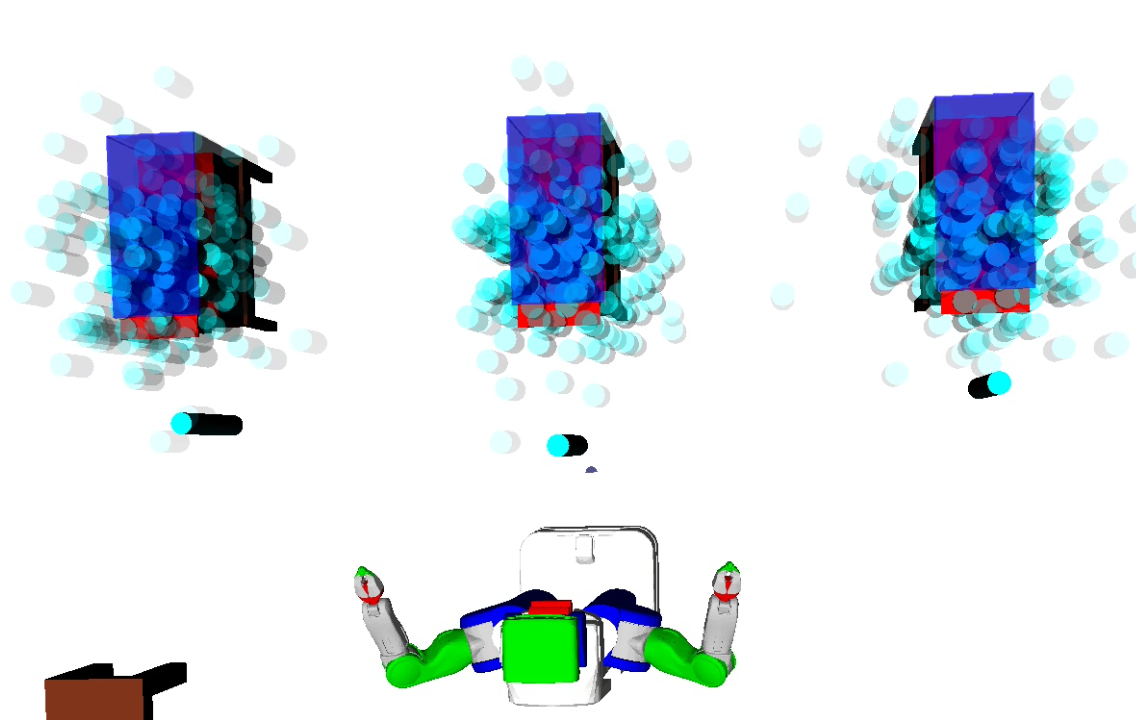
\includegraphics[width=\textwidth]{drawer_images/drawer_dist_0.png}
    \caption{}
    \label{fig:step1}
  \end{subfigure}
  \begin{subfigure}[b]{0.48\linewidth}
    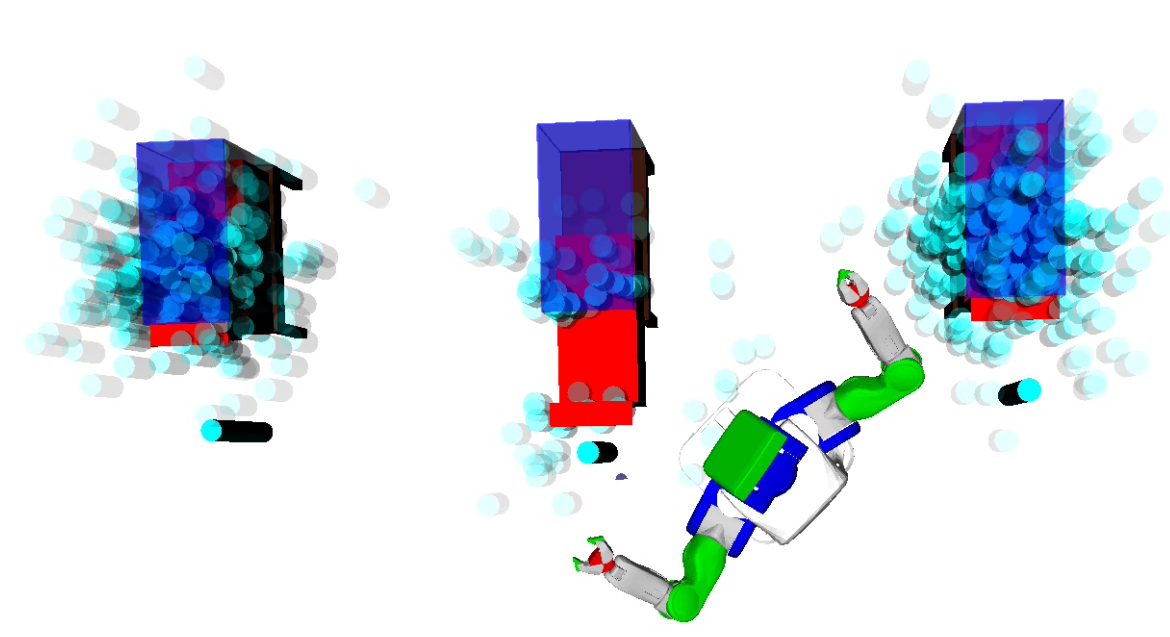
\includegraphics[width=\textwidth]{drawer_images/drawer_dist_1.png}
    \caption{}
    \label{fig:step2}
  \end{subfigure}
  \begin{subfigure}[b]{0.48\linewidth}
    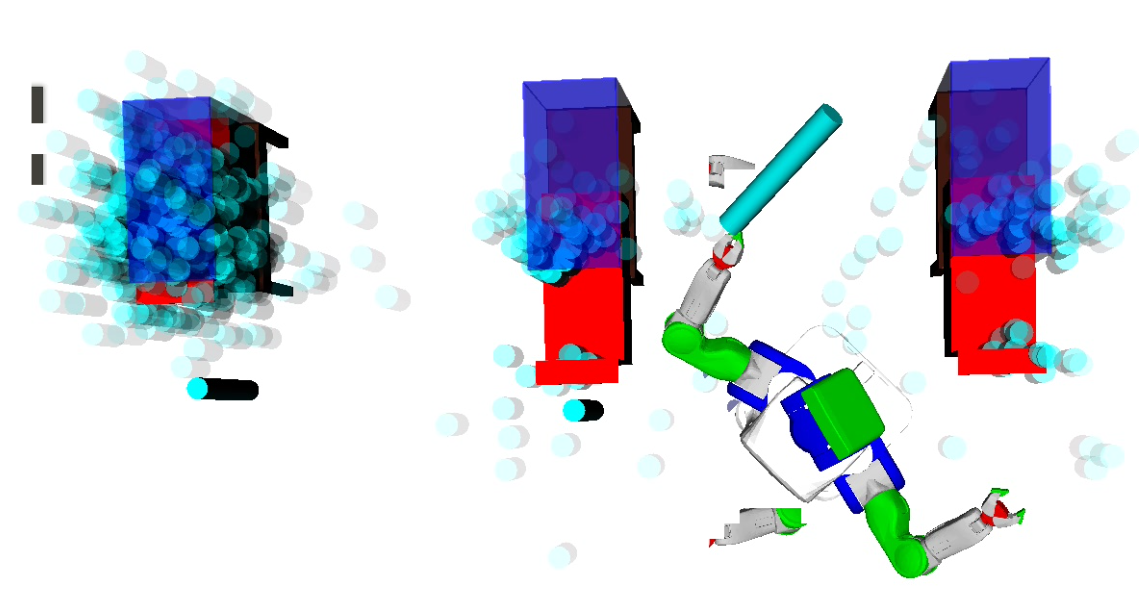
\includegraphics[width=\textwidth]{drawer_images/drawer_dist_2.png}
    \caption{}
    \label{fig:step4}
  \end{subfigure}
  \begin{subfigure}[b]{0.48\linewidth}
    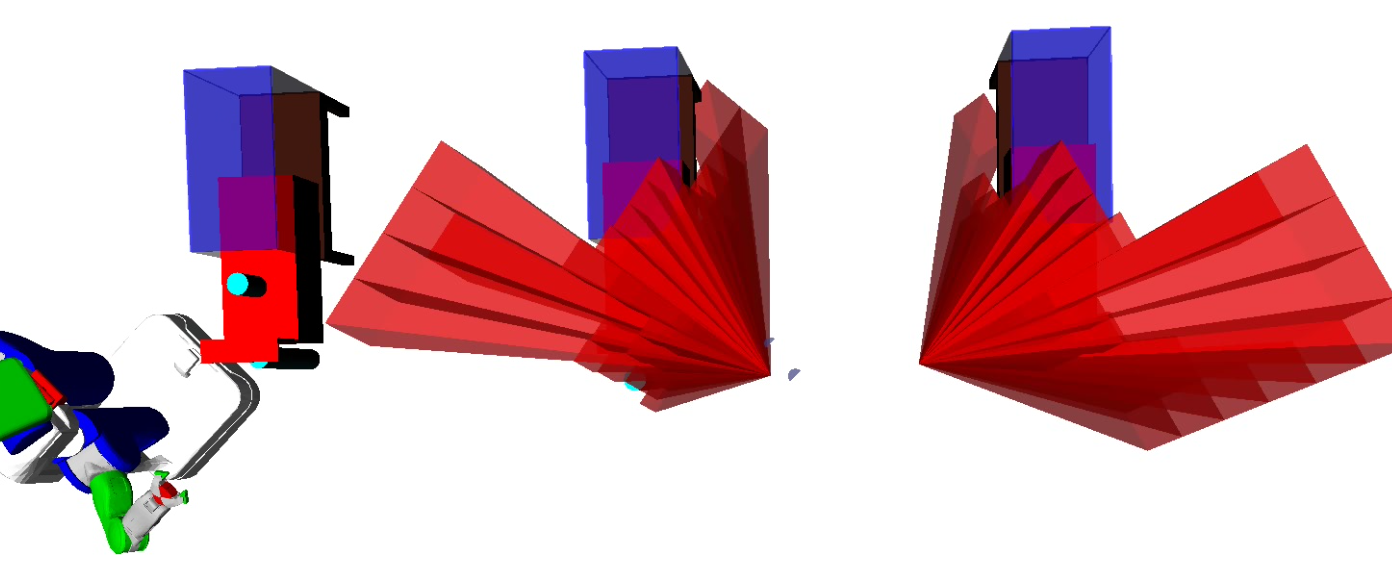
\includegraphics[width=\textwidth]{drawer_images/drawer_dist_negreg.png}
    \caption{}
    \label{fig:step5}
  \end{subfigure}
  %% \begin{subfigure}[b]{0.3\linewidth}
  %%   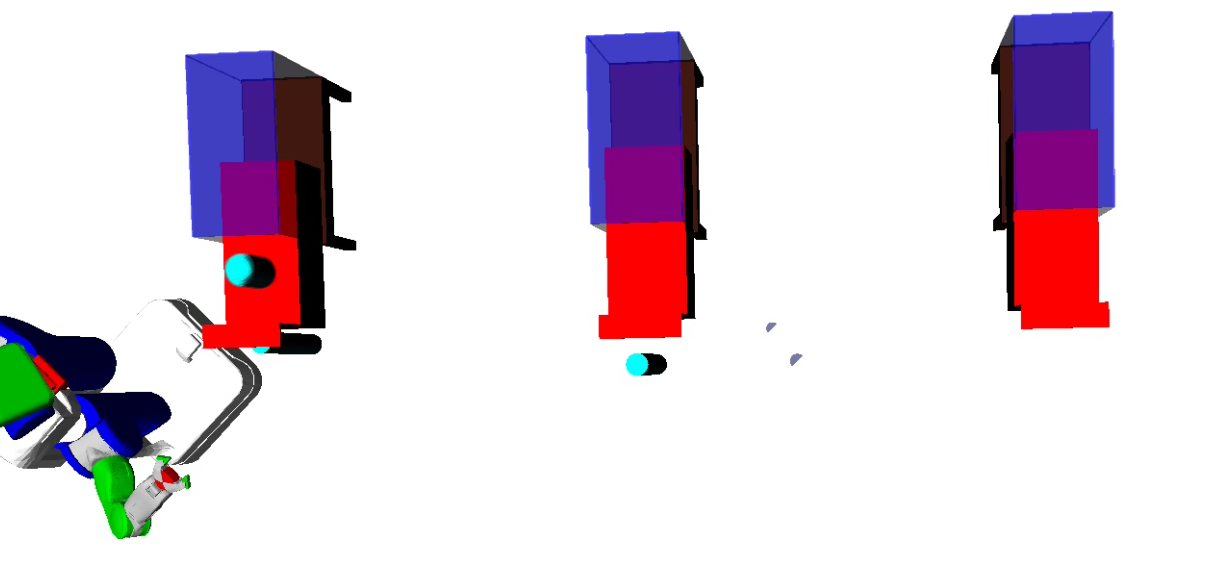
\includegraphics[width=\textwidth]{drawer_images/drawer_dist_3.png}
  %%   \caption{After observing three drawers (object was seen)}
  %%   \label{fig:step6}
  %% \end{subfigure}
  \caption{Intermediate belief states from a sample execution in our
    drawer search domain. We search for an object with a multimodal
    Gaussian distribution over three drawers. We illustrate beliefs with
    samples from the posterior distribution and show likelihoods with
    the transparency of objects. In this case, the object was in the
    leftmost drawer, and was found after searching the other
    drawers because they had a higher likelihood of containing the object. (a) shows the initial state and (b) and (c) show
    intermediate states at which we had to replan. Notice that we only clear
    the obstruction in front of the drawer when it is close enough to hinder sufficient opening.
    (d) shows the view cones from negative observations that were generated during planning.}
  \label{fig:drawerimgs}
\end{figure}

\begin{figure*}
  \centering
  \begin{subfigure}[b]{0.22\linewidth}
    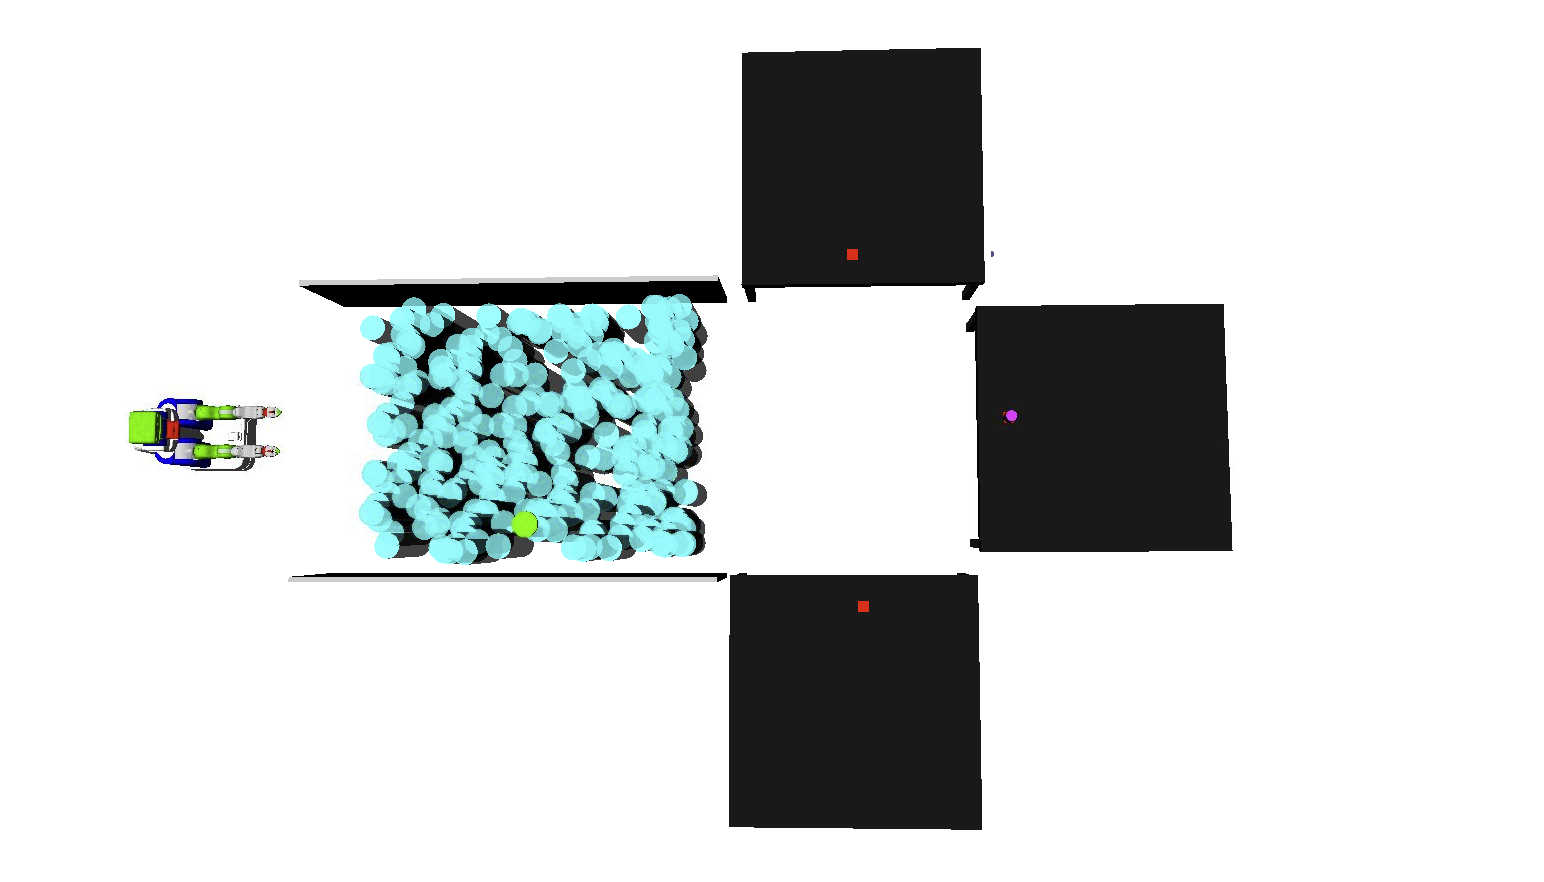
\includegraphics[width=\textwidth]{corridor_images/0-observe.png}
    \caption{Initial belief state}
    \label{fig:step1}
  \end{subfigure}
  \begin{subfigure}[b]{0.22\linewidth}
    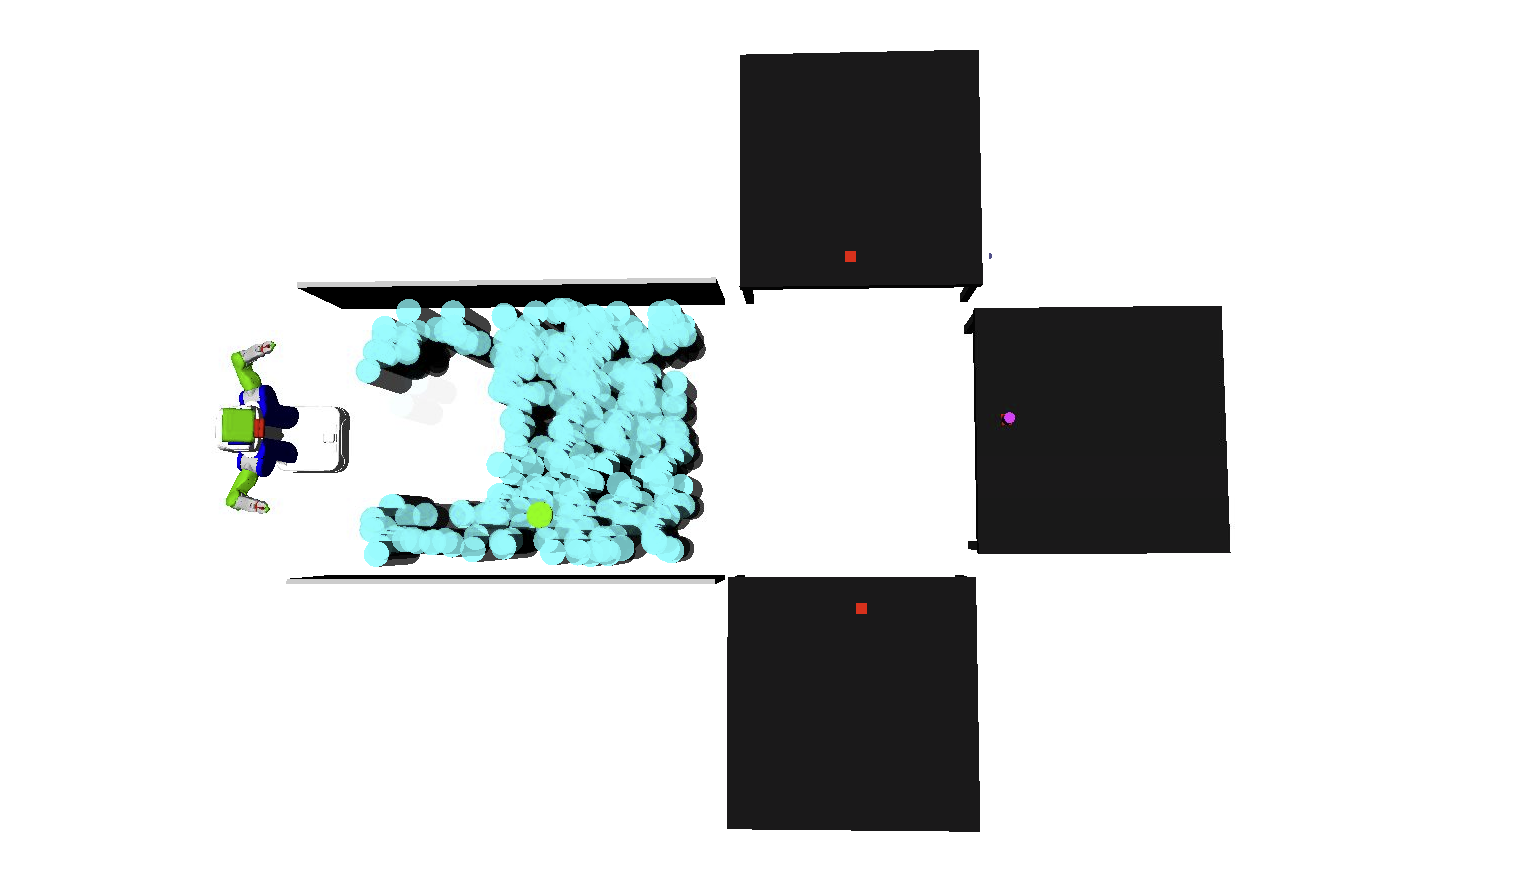
\includegraphics[width=\textwidth]{corridor_images/1-observe.png}
    \caption{After 1 observations}
    \label{fig:step2}
  \end{subfigure}
  \begin{subfigure}[b]{0.22\linewidth}
    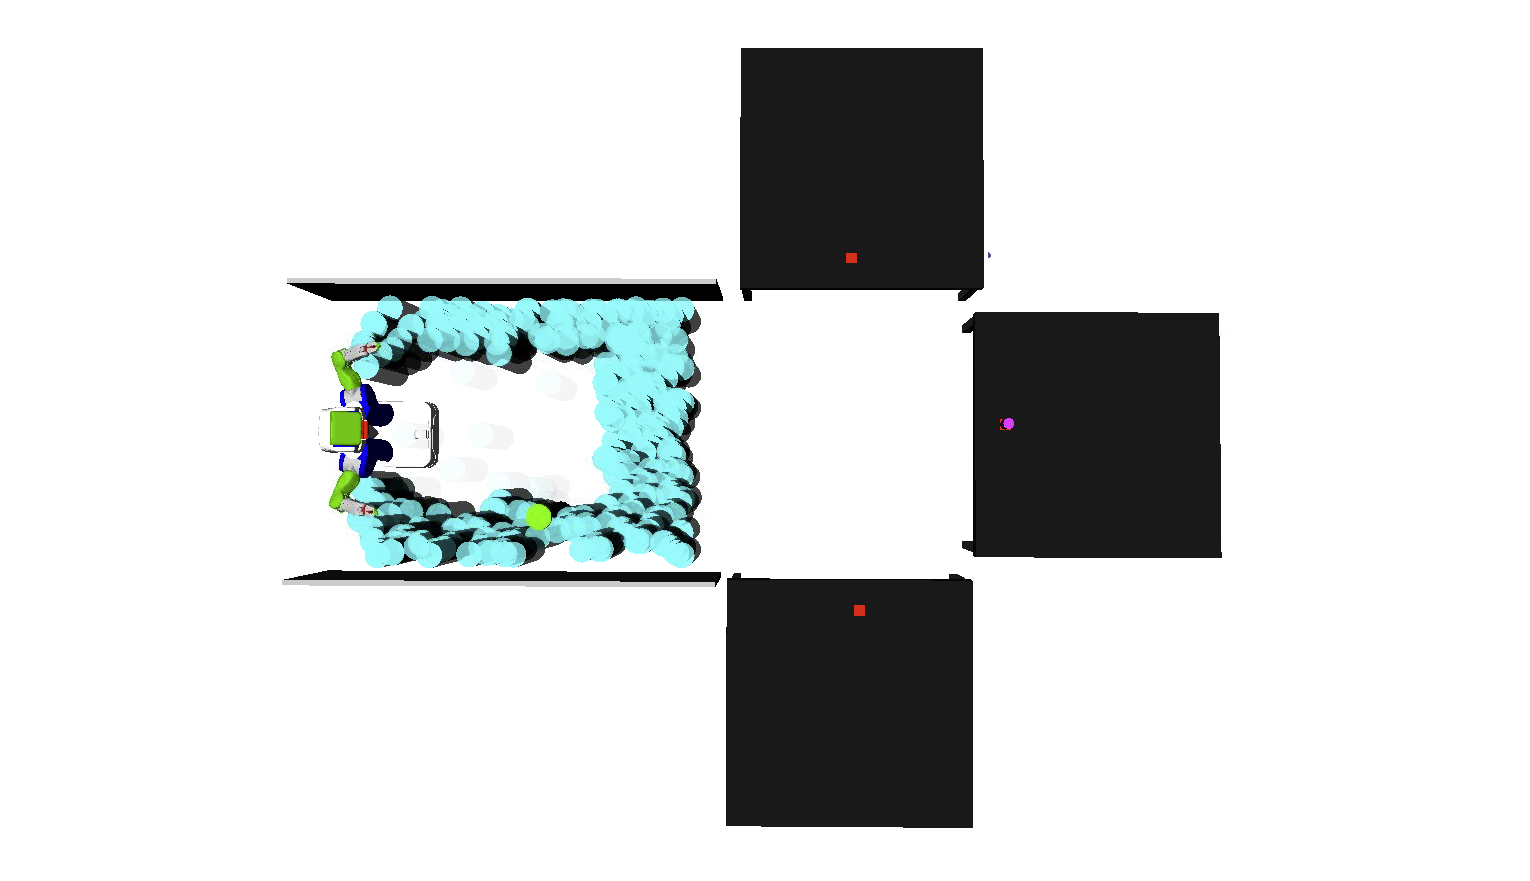
\includegraphics[width=\textwidth]{corridor_images/2-observe.png}
    \caption{After 2 observations}
    \label{fig:step3}
  \end{subfigure}
  \begin{subfigure}[b]{0.22\linewidth}
    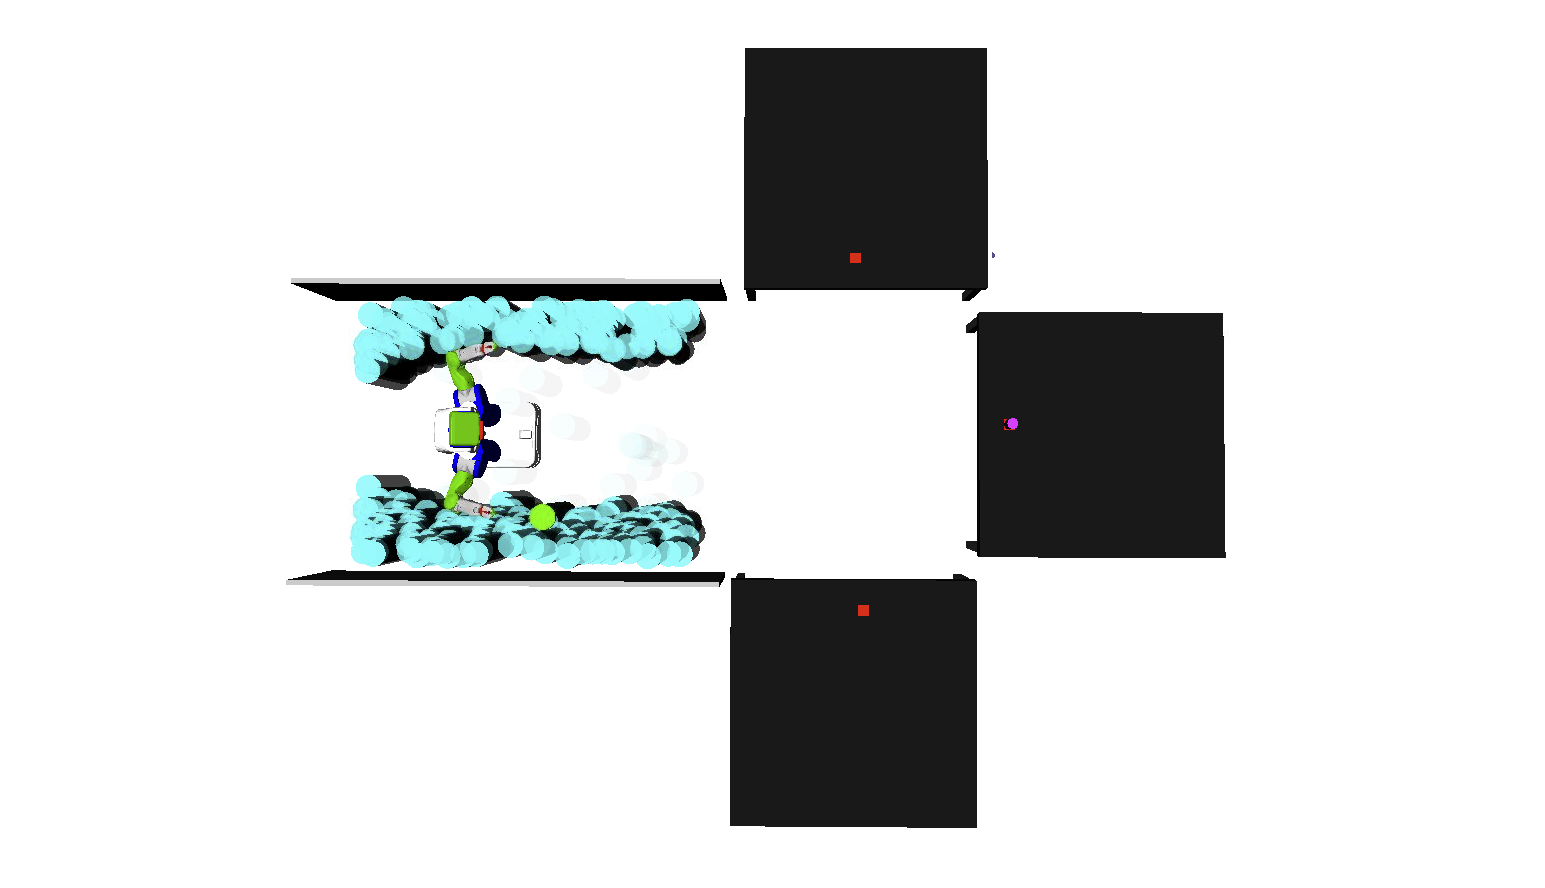
\includegraphics[width=\textwidth]{corridor_images/3-observe.png}
    \caption{After 3 observations}
    \label{fig:step4}
  \end{subfigure}
  \caption{Execution trace of interfaced belief space planning
    traversing a corridor with uncertain obstacles.
    The blue cylinders are drawn from the uniform belief distribution
    during execution. After reaching the other side of the corridor,
    the robot will pick up two target tables from the three tables.}
  \label{fig:corridorimgs}
\end{figure*}

We evaluate \ibsp{} in partially observable pick-and-place and navigation tasks.
The robot in our simulation is a full model of the Willow Garage PR2. We
provide results for several belief distributions: unimodal Gaussian, multimodal
Gaussian, and uniform.
\subsection{Observation Operator Specification and Generators}
The maximum likelihood component of the determinized problem
essentially follows the dynamics specified in
\secref{sec-formulation}. In order to extend this domain to handle
partial observability, we add the following fluents and operators:
\begin{tightlist}
  \item[]Fluents: \\\emph{MLInView}(r\_pose, o\_pose\_bel)\\
    \emph{MLOccludes}(obj, o\_pose\_bel, r\_obs\_pose)\\
    \emph{MLObstructs}(obj, traj)\\
    \emph{UncertainGP}(o\_pose\_bel, r\_pose, grasp)\\
    \emph{UncertainObstructs}(obj, traj)
  \item[]Operators:
  \begin{tightlist} \item \emph{ObserveGP}(r\_obs\_pose, o, o\_pose\_bel)
\begin{tightlist}
  \item[\emph{pre}:] \emph{MLLoc}(o, o\_pose\_bel) $\wedge$
    \emph{MLRLoc}(r\_obs\_pose) \\$\wedge$ $\forall o_i
    \lnot$\emph{MLOccludes}($o_i$, o\_pose\_bel, r\_obs\_pose) \\ $\wedge$
    \emph{MLInView}(r\_obs\_pose, o\_pose)
  \item[\emph{eff}:] $\forall$ r\_p, g $\lnot$\emph{UncertainGP}(o\_pose\_bel, r\_p, g)
\end{tightlist}
\item  \emph{ObserveTrajectory}(r\_obs\_pose, traj) 

\begin{tightlist}
  \item[\emph{pre}:] \emph{MLRLoc}(r\_obs\_pose) \\$\wedge$
    \emph{MLInView}(r\_obs\_pose, traj)\\ $\wedge$
    $\forall o_i \lnot$\emph{MLOccludes}($o_i$, traj, r\_obs\_pose)\\ $\wedge$
    $\forall o_i \lnot$\emph{MLObstructs}(obj, traj)
  \item[\emph{eff}:] $\forall o_i \lnot$\emph{UncertainObstructs}($o_i$,
    traj)
\end{tightlist}
\end{tightlist}
\end{tightlist}

The additional skolem functions needed to support this functionality
are \emph{ViewPose}(Obj) and \emph{ViewPose}(Traj) for each object and
trajectory reference. The generator for object view poses draws
samples from a 1-meter unit disc around the object, and the head pose
is fixed to point at the object's maximum likelihood position. The
generator for trajectory view poses returns the first step along the
trajectory that has non-negligible probability of being in
collision. To observe the uncertain step, a viable base pose is
sampled from regions with negligible collision probability along the
same trajectory.

\subsection{Observation model and state estimation for the PR2}
We model observations with ray casting from a simulated head-mounted
Kinect on our robot. For objects that are in the view
frustum, we get a false negative with probability proportional to the
amount of the object that is occluded. If we do get a positive
observation, we observe the object's true pose with Gaussian noise.


In order to successfully plan for this domain, it is important that we
effectively incorporate negative observations into our
updates. Without these negative observations, it is impossible to determine
if a trajectory is clear without observing actual objects
locations. 

We account for negative observations with a factored representation
for the belief state. In one component, we maintain a distribution
that accounts for positive observations (e.g., a Kalman filter). The
other component is an explicit representation of the view cones
associated with negative observations. We refer to the first component
as the positive observation distribution and the second as the
negative regions. To sample from this distribution, we perform
probabilistic rejection sampling: sample from the positive observation
distribution and then discard the sample in inverse proportion to the
probability that it lies in a negative region. The inverse
probability is given by $\max(1,\dfrac{\text{penetration
    depth}}{\text{object radius}})$, where penetration depth is the
minimum translation distance that takes two objects out of collision and object
radius is found by approximating the object as a sphere.


\subsection{Evaluations}
We implement our experiments in Python and use
OpenRave~\cite{Diankov_2008_6117} to represent the environment. We use
trajectory optimization for our motion planning~\cite{schulman2013finding}
and implement custom collision checking in Flexible Collision Library~\cite{jia2014fcl} to handle
collisions. We use the Fast-Forward and Fast-Downward
task planners to solve our high-level planning problems. Because our system works
independently of the chosen task planner, we use Fast-Forward in domains involving negative
preconditions, which are not supported by Fast-Downward. Experiments were run in series on
Intel Core i7-4770K machines with 16GB RAM. We validate our approach in three distinct scenarios.

To explore ensuring safety in robot navigation tasks under uncertainty, we
evaluate performance in a corridor domain. We place the robot at one end of a corridor
and present it with the goal of traversing the corridor, then grasping
objects on tables on the other side. Uniform distributions model the locations of
a varying number of obstructing columns throughout the corridor; thus, the solution
typically ends up as an alternating sequence of observations and motions. Note that this task would be essentially
insoluble without accounting for negative observations appropriately.

The second task demonstrates the ability to reason about occlusions. We
set a goal of grasping a target object from a cluttered table with other
objects on it: some have deterministic locations and others have a Gaussian distribution
modeling their location. The target object's location is also drawn from a Gaussian
distribution. \ibsp{} plans to remove any occlusions, to observe the target object, and
then to pick it up. In our experiments, we maintain that 3 of the objects on the table -- always including
the target object -- are part of the belief space.

In our final scenario, the robot has lost its keys and is trying to locate them among three drawers they could be in.
This setup illustrates multimodal planning behavior with a mixture of Gaussians as the prior for the target's location.
Furthermore, we introduce a deterministic object in front of each drawer, which possibly
obstructs it from being opened. \ibsp{} begins by assuming the target is placed at its maximum likelihood
location; accordingly, it discovers that the target is obstructed by the drawer containing it, then
plans to open this drawer. If the outer deterministic object impedes the drawer from opening, this
obstruction fact is also discovered and accounted for. During execution, upon performing an observation inside the drawer, our system
chooses to refine the plan if the object was not actually seen (indicating that its true location is in another drawer).
The new refinement incorporates this negative observation, and the system may then try opening another drawer.

Table \ref{table:results} shows timing results for the three described
tasks. \figref{fig:drawerimgs} and \figref{fig:corridorimgs} show intermediate steps and belief
states for the drawer and corridor tasks. The included video demonstrates plan execution for all three tasks.


\begin{table}
  \centering
  \vspace{8pt}
  \tabcolsep=0.11cm{
  \begin{tabular}{cccc}
    \toprule
      Problem Type & \% Solved & Avg Time (s) & Avg \# Planner Runs\\
    \midrule
      Uni. corridor, 1 obj & 100 & 232 & 1.88\\
    \midrule
      Uni. corridor, 2 obj & 100 & 445 & 2.45\\
    \midrule
      Uni. corridor, 3 obj & 88 & 926 & 2.78\\
    \midrule
      Uni. corridor, 4 obj & 58 & 1168 & 2\\
    \midrule
      Table, 5 obj & 95 & 89 & 2.2\\
    \midrule
      Table, 10 obj & 95 & 162 & 2.21\\
    \midrule
      Table, 15 obj & 83 & 135 & 2.26\\
    \midrule
      Table, 20 obj & 70 & 229 & 2.03\\
    \midrule
      Table, 25 obj & 68 & 166 & 1.84\\
    \midrule
      Table, 30 obj & 48 & 122 & 1.96\\
    \midrule
      3-Drawer search & 93 & 325 & 2.11\\
    \bottomrule
  \end{tabular}}
  \caption{Solution percentages, running times, and number of high-level planner calls for \ibsp{} in
    occluded search and navigation tasks. Unimodal cluttered table results are from 40
    randomly generated problems per number of objects. Multimodal 3-drawer search results
    are from 30 iterations. Uniform corridor navigation results are from 40 random locations of corridor obstructions, per number of objects. Time limit: 1800s.}
  \label{table:results}
\end{table}




\section{Conclusion}
We presented a novel approach to combining task and motion planning
in belief space through the \emph{maximum likelihood determinization}
principle. We evaluated our algorithm on several domains, where it completed
challenging sequences of perception and geometric reasoning by task planning in
an abstract representation of the problem. Potential future work includes experimenting on a real PR2, incorporating noisy transition models between environment states, and answering maximum likelihood queries using methods other than Monte Carlo sampling (e.g. SQP).

%\addtolength{\textheight}{-12cm}   % This command serves to balance the column lengths
                                  % on the last page of the document manually. It shortens
                                  % the textheight of the last page by a suitable amount.
                                  % This command does not take effect until the next page
                                  % so it should come on the page before the last. Make
                                  % sure that you do not shorten the textheight too much.

%%%%%%%%%%%%%%%%%%%%%%%%%%%%%%%%%%%%%%%%%%%%%%%%%%%%%%%%%%%%%%%%%%%%%%%%%%%%%%%%



%%%%%%%%%%%%%%%%%%%%%%%%%%%%%%%%%%%%%%%%%%%%%%%%%%%%%%%%%%%%%%%%%%%%%%%%%%%%%%%%



%%%%%%%%%%%%%%%%%%%%%%%%%%%%%%%%%%%%%%%%%%%%%%%%%%%%%%%%%%%%%%%%%%%%%%%%%%%%%%%%
\bibliography{latex_files/references}

\end{document}
